\chapter{Results}

This section will discuss the contributions from this thesis.
Then it dives into some of the data required for a tree editor.
Next is a presentation of the prototypes and their results, with regards to the research questions.
Finally, a list of requirements and an architecture for a Tree Editor is presented.

\section{Contribution}

This thesis will provide an overview of the developments in \gls{cloud} \glspl{IDE} with regards to modeling in \gls{emf}.
An analysis of the data will show how existing tools and architectures can be applied in a new \gls{cloud} \gls{IDE} for \gls{Ecore} modeling.

Additionally, a foundation for a \emph{software product} will be presented.
The foundations will be built further upon in a master's thesis.
The foundations are a set of software requirements and an initial architecture for a \gls{cloud} based \gls{Ecore} Tree editor inside an existing \gls{cloud} \gls{IDE}.


\section{Extensible Integrated Development Environments}

This section will discuss the technologies and mechanisms found during data collection that are relevant for a solution.

\subsection{Integrated Development Environments}\label{sec:editors}

This section will describe the most relevant \acrfullpl{IDE} for \acrlong{emf} and the \gls{cloud}.

\subsubsection{Visual Studio Code}\label{sec:vscode}

\paragraph*{What it is}
Visual Studio Code (\gls{VSCode}) is a text editor and \acrfull{IDE} created by
Microsoft. The VSCode editor is based on the \gls{open source}\footnote{Source for VSCode is available at \href{https://github.com/microsoft/vscode}{https://github.com/microsoft/vscode}} software (OSS) called \emph{VS Code Project}.~\cite{helmingEclipseTheiaIDE2019} 
The VSCode editor has Microsoft-specific customizations, which makes it slightly different from the OSS project.~\cite{MicrosoftVscode2020} (This is analogous to the relationship between the \gls{open source} Chromium and the proprietary Google Chrome.)

\begin{figure}[htbp]
  \centering
  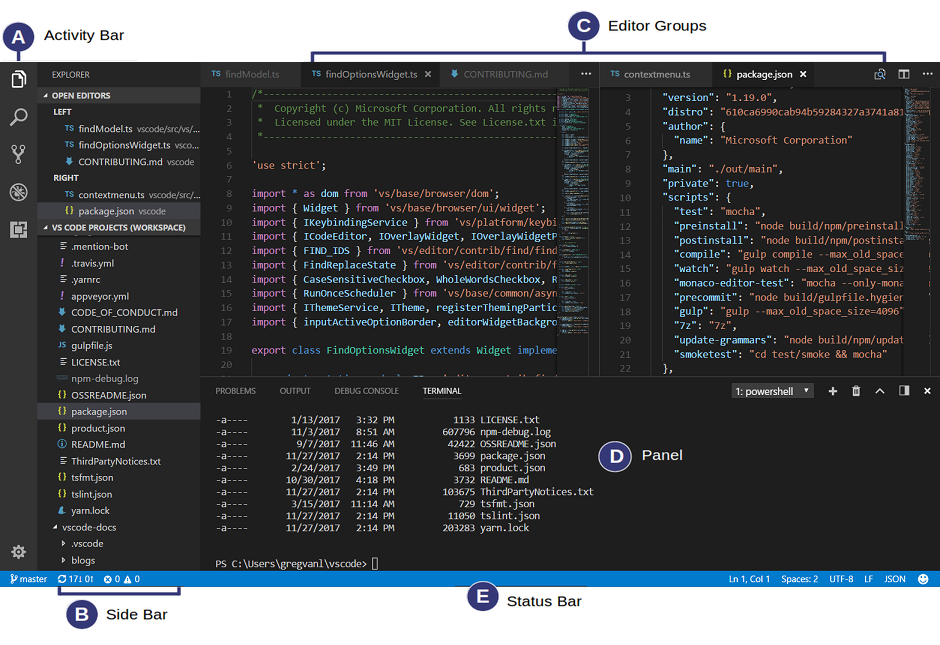
\includegraphics[width=\textwidth]{figures/vscode-ui}
  \caption[Visual Studio Code User Interface]{The user interface of Visual Studio Code, with annotations for the different components (\emph{A-E}).\cite{microsoftVisualStudioCode2020}}\label{fig:vscode-ui}
\end{figure}

\paragraph*{Intended use} Primarily an editor for textual programming languages.
VSCode has no support for diagrams or binary file viewers (like 3D models) out of the box (except pictures like \texttt{png} etc.). By default, it supports \texttt{Javascript}, \texttt{Typescript} and \texttt{Markdown}; common technologies related to web development.
VSCode can be extended to support other languages and editors, see \cref{sec:vscode-extension}.

% What does it do?
% Who made it?
% Architecture

\paragraph*{Architecture}
VSCode runs as a desktop application, and uses Electron and javascript for its runtime.
The architecture is centered on a \emph{core} which loads \emph{extensions}.
The core is shown in \cref{fig:vscode-layers-architecture}, and is split internally into \emph{layers} with different responsibilies.
Each layer is again organized based on the target runtime, like \emph{browser} or \emph{\gls{Electron}}, as seen in \cref{fig:vscode-component-architecture}.
The actual text editor in \gls{VSCode} is called \emph{Monaco}, and is available as a standalone package.~\cite{benjaminpaseroSourceCodeOrganization2020}


\begin{figure}[htbp]
  \centering
  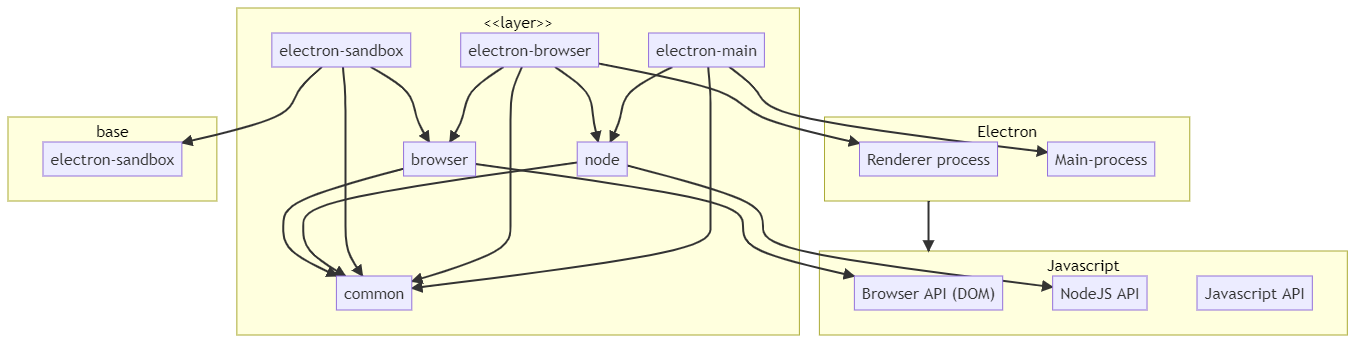
\includegraphics[width=\textwidth]{figures/vscode-component-architecture}
  \caption[VSCode component Architecture]{The internal architecture of each component in VSCode. The \texttt{<<layer>>} label represents each of the layers in \cref{fig:vscode-layers-architecture}, like \emph{base} or \emph{platform}. Every layer is organized by runtime dependencies.~\cite{benjaminpaseroSourceCodeOrganization2020}}\label{fig:vscode-component-architecture}
\end{figure}

\begin{figure}[htbp]
  \centering
  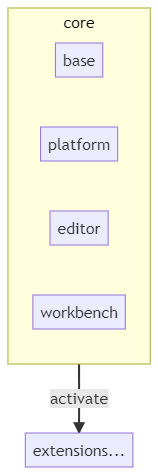
\includegraphics[width=2cm]{figures/vscode-layers-architecture}
  \caption[VSCode Layers]{The internal layers which the VSCode \texttt{core} is separated into.~\cite{benjaminpaseroSourceCodeOrganization2020}}\label{fig:vscode-layers-architecture}
\end{figure}



\subsubsection{Theia}\label{sec:theia}

\paragraph*{What it is}
\Gls{Theia} is an editor like \gls{VSCode}, but designed from the start to work in web browsers.
A screenshot is shown in \cref{fig:theia-user-interface}; notice how it is almost identical to \gls{VSCode}.
The project was originally started by TypeFox, and then donated to the Eclipse Foundation.
It is free and fully \gls{open source}\footnote{Source for Theia is available at \href{https://github.com/eclipse-theia/theia/}{https://github.com/eclipse-theia/theia/}}.
\Gls{Theia} is based on some of the same components as \gls{VSCode}, and uses Monaco as well.
The main uses of Theia now is as an editor for workspace software like \gls{Che} and \gls{Gitpod}.
Theia supports VSCode extensions, but not all of the \acrshortpl{API} in VSCode are implemented yet\footnote{A table of \acrshort{API} support is provided at \href{https://che-incubator.github.io/vscode-theia-comparator/status.html}{https://che-incubator.github.io/vscode-theia-comparator/status.html}.}.

\begin{figure}[htbp]
  \centering
  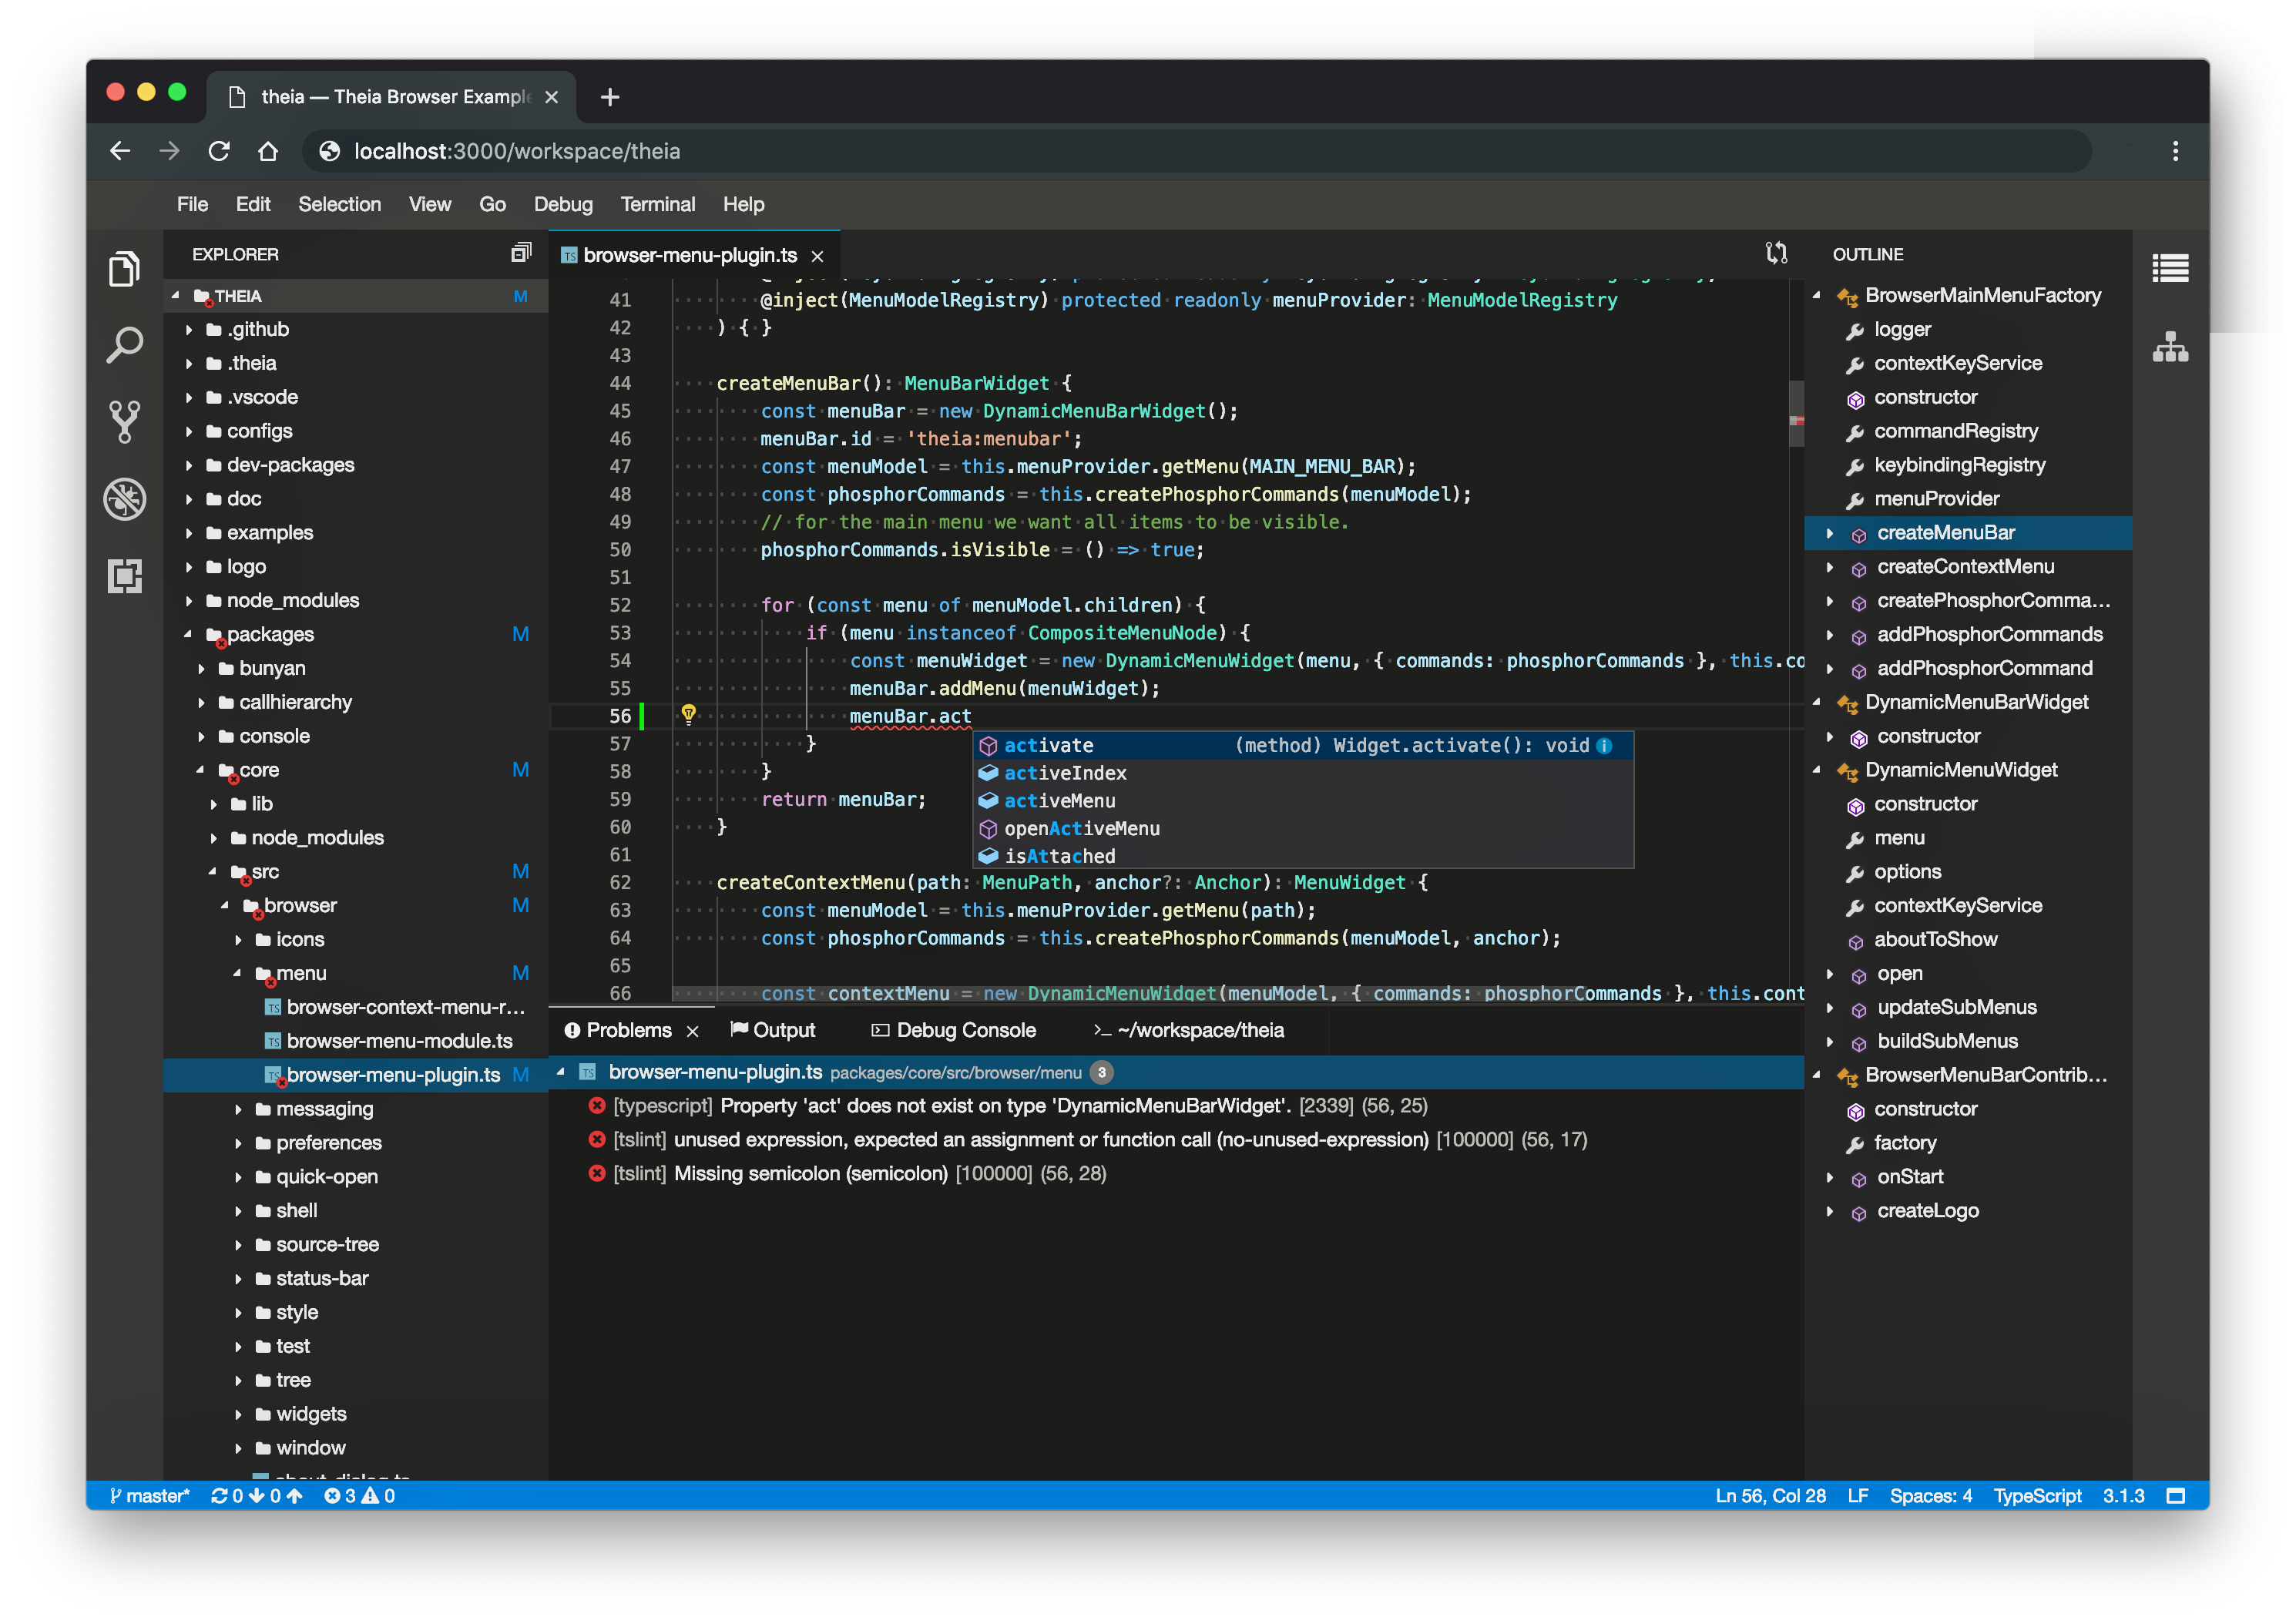
\includegraphics[width=\textwidth]{figures/theia-screenshot.png}
  \caption[Theia User Interface]{A screenshot of the Theia user interface.~\cite{eclipsefoundationEclipsetheiaTheia2020}}\label{fig:theia-user-interface}
\end{figure}

\paragraph*{Intended use}
\Gls{Theia} was created to be a framework for creating custom and
white-labeled \acrshortpl{IDE} and tools. Theia itself was not an IDE.~\cite{helmingEclipseTheiaIDE2019}

\paragraph*{Architecture --- runtime}
The architecture of Theia is similar to \gls{VSCode}.
The biggest difference is in the runtime.
\Gls{Theia} is split into a backend and frontend process. 
The backend \textit{could} run remotely, or locally. 
The frontend is \gls{Electron} or a browser.
The backend and frontend communicate with \gls{JSON-RPC} over \glspl{WebSocket} or \gls{REST}/HTTP\@. 
Both the frontend and backend source codes are heavily architected around
\emph{dependency injection}.
The backend runs an \texttt{ExpressJs} web server which serves code to the frontend (see \cref{fig:theia-communication}).~\cite{typefoxArchitectureOverview}

The frontend can always assume it has \texttt{browser API}, but not
\texttt{NodeJS}/\texttt{Electron} \gls{API}.~\cite{typefoxArchitectureOverview}

To support different programming languages, the backend talks over the \acrfull{LSP} with different \emph{language servers}.
One backend process serves one workspace/user.
Multiple clients can connect, but they will all share the same workspace.~\cite{MultiLanguageIDEImplemented2017}

\begin{figure}[htbp]
  \centering
  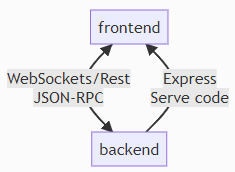
\includegraphics[width=4cm]{figures/theia-api.png}
  \caption[Theia frontend and backend communication]{Theia serves the frontend with ExpressJs and communicates between the frontend and backend with JSON-RPC.}\label{fig:theia-communication}
\end{figure}

\paragraph*{Architecture --- components}
\Gls{Theia} uses a extension oriented design.
This means that almost all functionality is provided as a \emph{Theia Extension} (see \cref{sec:theia-extension}).
For example, the \acrshortpl{API} for user-installable \emph{Theia Plugins} (see \cref{sec:theia-plugin}) are provided as an extension.
The \emph{Monaco} editor from \gls{VSCode} is also provided by an extension.
The main components of Theia is shown in \cref{fig:theia-components}.
(Note that this diagram is from 2017 and could be outdated).
The components are separated into frontend, backend and external (blue).
External resources could be processes for language compilation, package managers, terminal shells etc..

Of particular interest is the \texttt{Extensions} component with \texttt{Inversify.js}. This is the dependency injection mechanism which loads other extensions into Theia. (Also note that the \texttt{Plugin} extension for \gls{VSCode} extensions is missing in this diagram. That component was added later by RedHat\footnote{RedHat chose to use Theia in \gls{Che}, and wanted plugins that could be installed by users during run-time. They opted for the \gls{VSCode} extension mechanism for this.}.)

\begin{figure}[htbp]  % order of priority: h here, t top, b bottom, p page
  \centering
  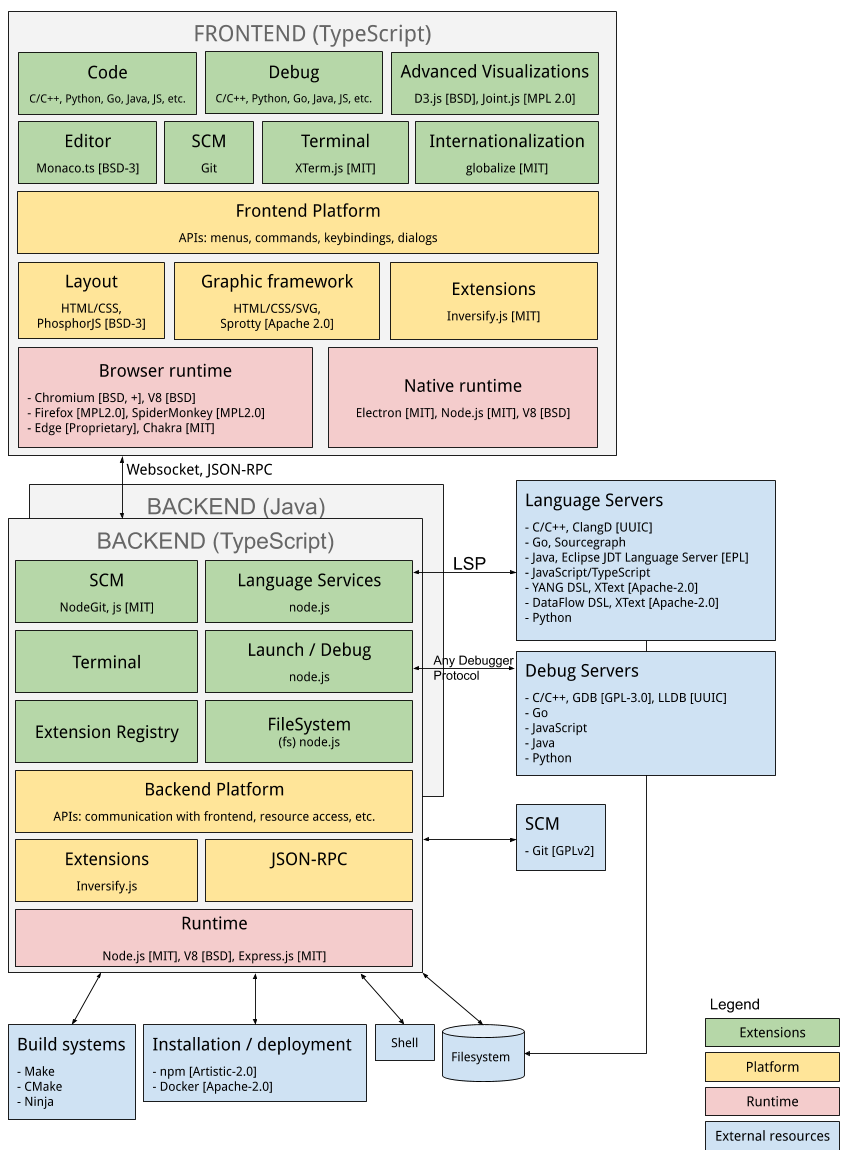
\includegraphics[width=\textwidth]{figures/Multi-Language-IDE-implemented-in-JS-Scope-and-Architecture}
  \caption[Theia module Architecture]{The main components in Theia. Some components have third party libraries, languages or runtimes listed under their component name, as examples. The figure is from a design document made in 2017, and could be outdated. (The author is unknown, but assumed to be a TypeFox employee. The document is linked to on the official Theia website).~\cite{MultiLanguageIDEImplemented2017}}\label{fig:theia-components}
\end{figure}

\paragraph*{Architecture --- code organization}
Every extension in Theia is organized based on the runtime dependencies.
This is similar to how \gls{VSCode} does it.
See \cref{fig:theia-organization}. The main difference is \texttt{electron-sandbox} in \gls{VSCode} and \texttt{electron-main} in Theia.
Every Theia extension can also provide two entrypoints: \texttt{frontend} and \texttt{backend}. This allows extensions to provide different code for the different parts of Theia (see \cref{sec:theia-extension}).

\begin{figure}[htbp]  % order of priority: h here, t top, b bottom, p page
  \centering
  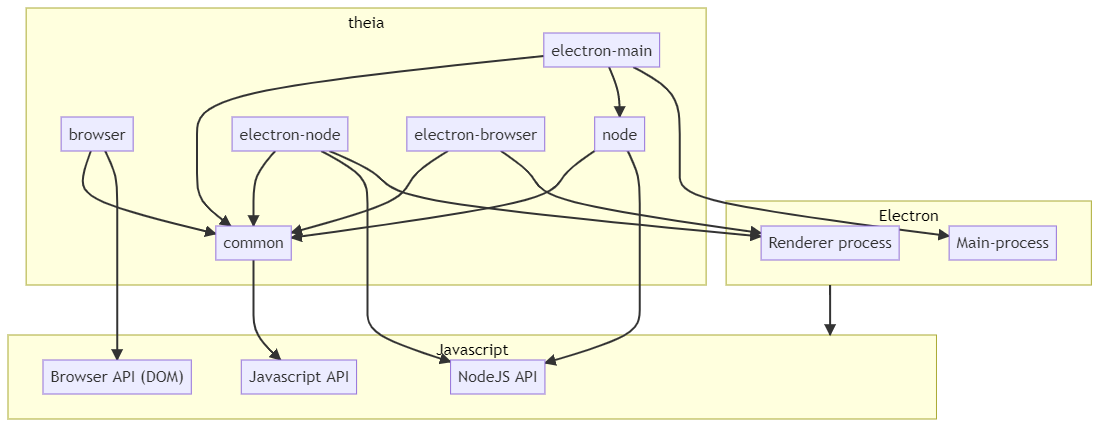
\includegraphics[width=\textwidth]{figures/theia-code-organization}
  \caption[Theia code organization]{The code in Theia extensions are organized based on the dependency on runtime \acrshortpl{API}. The box named \texttt{theia} represents an extension in Theia.~\cite{antonkosyakovCodeOrganization2019}}\label{fig:theia-organization}
\end{figure}

% What does it do?
% Who made it?
% Architecture

\subsubsection{Eclipse IDE}\label{sec:eclipse-ide}
% What does it do?
% Who made it?
% Architecture

\paragraph*{What it is}
One of the older \glspl{IDE}. 
Originally desktop based, but some web frontends have been made (like \gls{RAP}).
Popular for java development and the main \gls{IDE} used by \gls{emf}.
It also serves as a framework for building user interfaces, as in \gls{RCP} and generated model editors (from genmodel).

\paragraph*{Intended use}
\Gls{Eclipse} is intended to be used as a \gls{IDE} and also framework for desktop based editors via \gls{RCP}.
It is very flexible, with support for addons/plugins that extend its capabilities.

\paragraph*{Architecture}
The \gls{Eclipse} is based on a core platform that loads other plugins and features to extend itself.
The core mechanism is OSGi and plugin manifests, along with Eclipse's extension points.
OSGi will load plugins and use dependency injection to connect components together.
The extension points are predefined areas of the \acrshort{IDE} where plugins can add functionality.
Plugins can also expose their own contribution points.
The plugin manifest specifies where a plugin will contribute, like which extension points should be added to.

\subsubsection{Coffee Editor IDE}\label{sec:coffee-ide}

\paragraph*{What it is}
The \emph{Coffee Editor IDE} is an example and reference implementation for a \gls{Theia}-based \gls{IDE}.
It uses Theia as its core, but adds more functionality through extensions (see \cref{sec:theia-extension}).
The Coffee Editor IDE has a graphical editor based on \gls{GLSP}, a form based editor using JSON-Forms (see \cref{sec:json-forms}), a tree editor using Theia Tree Editor (see \cref{sec:theia-tree-editor}), textual \acrshort{DSL} using XText (see \cref{sec:xtext}) and \gls{LSP} (see \cref{sec:lsp}).
An illustration of the Coffee Editor IDE is shown in \cref{fig:coffee-editor-overview}.

\begin{figure}[htbp] 
  \centering
  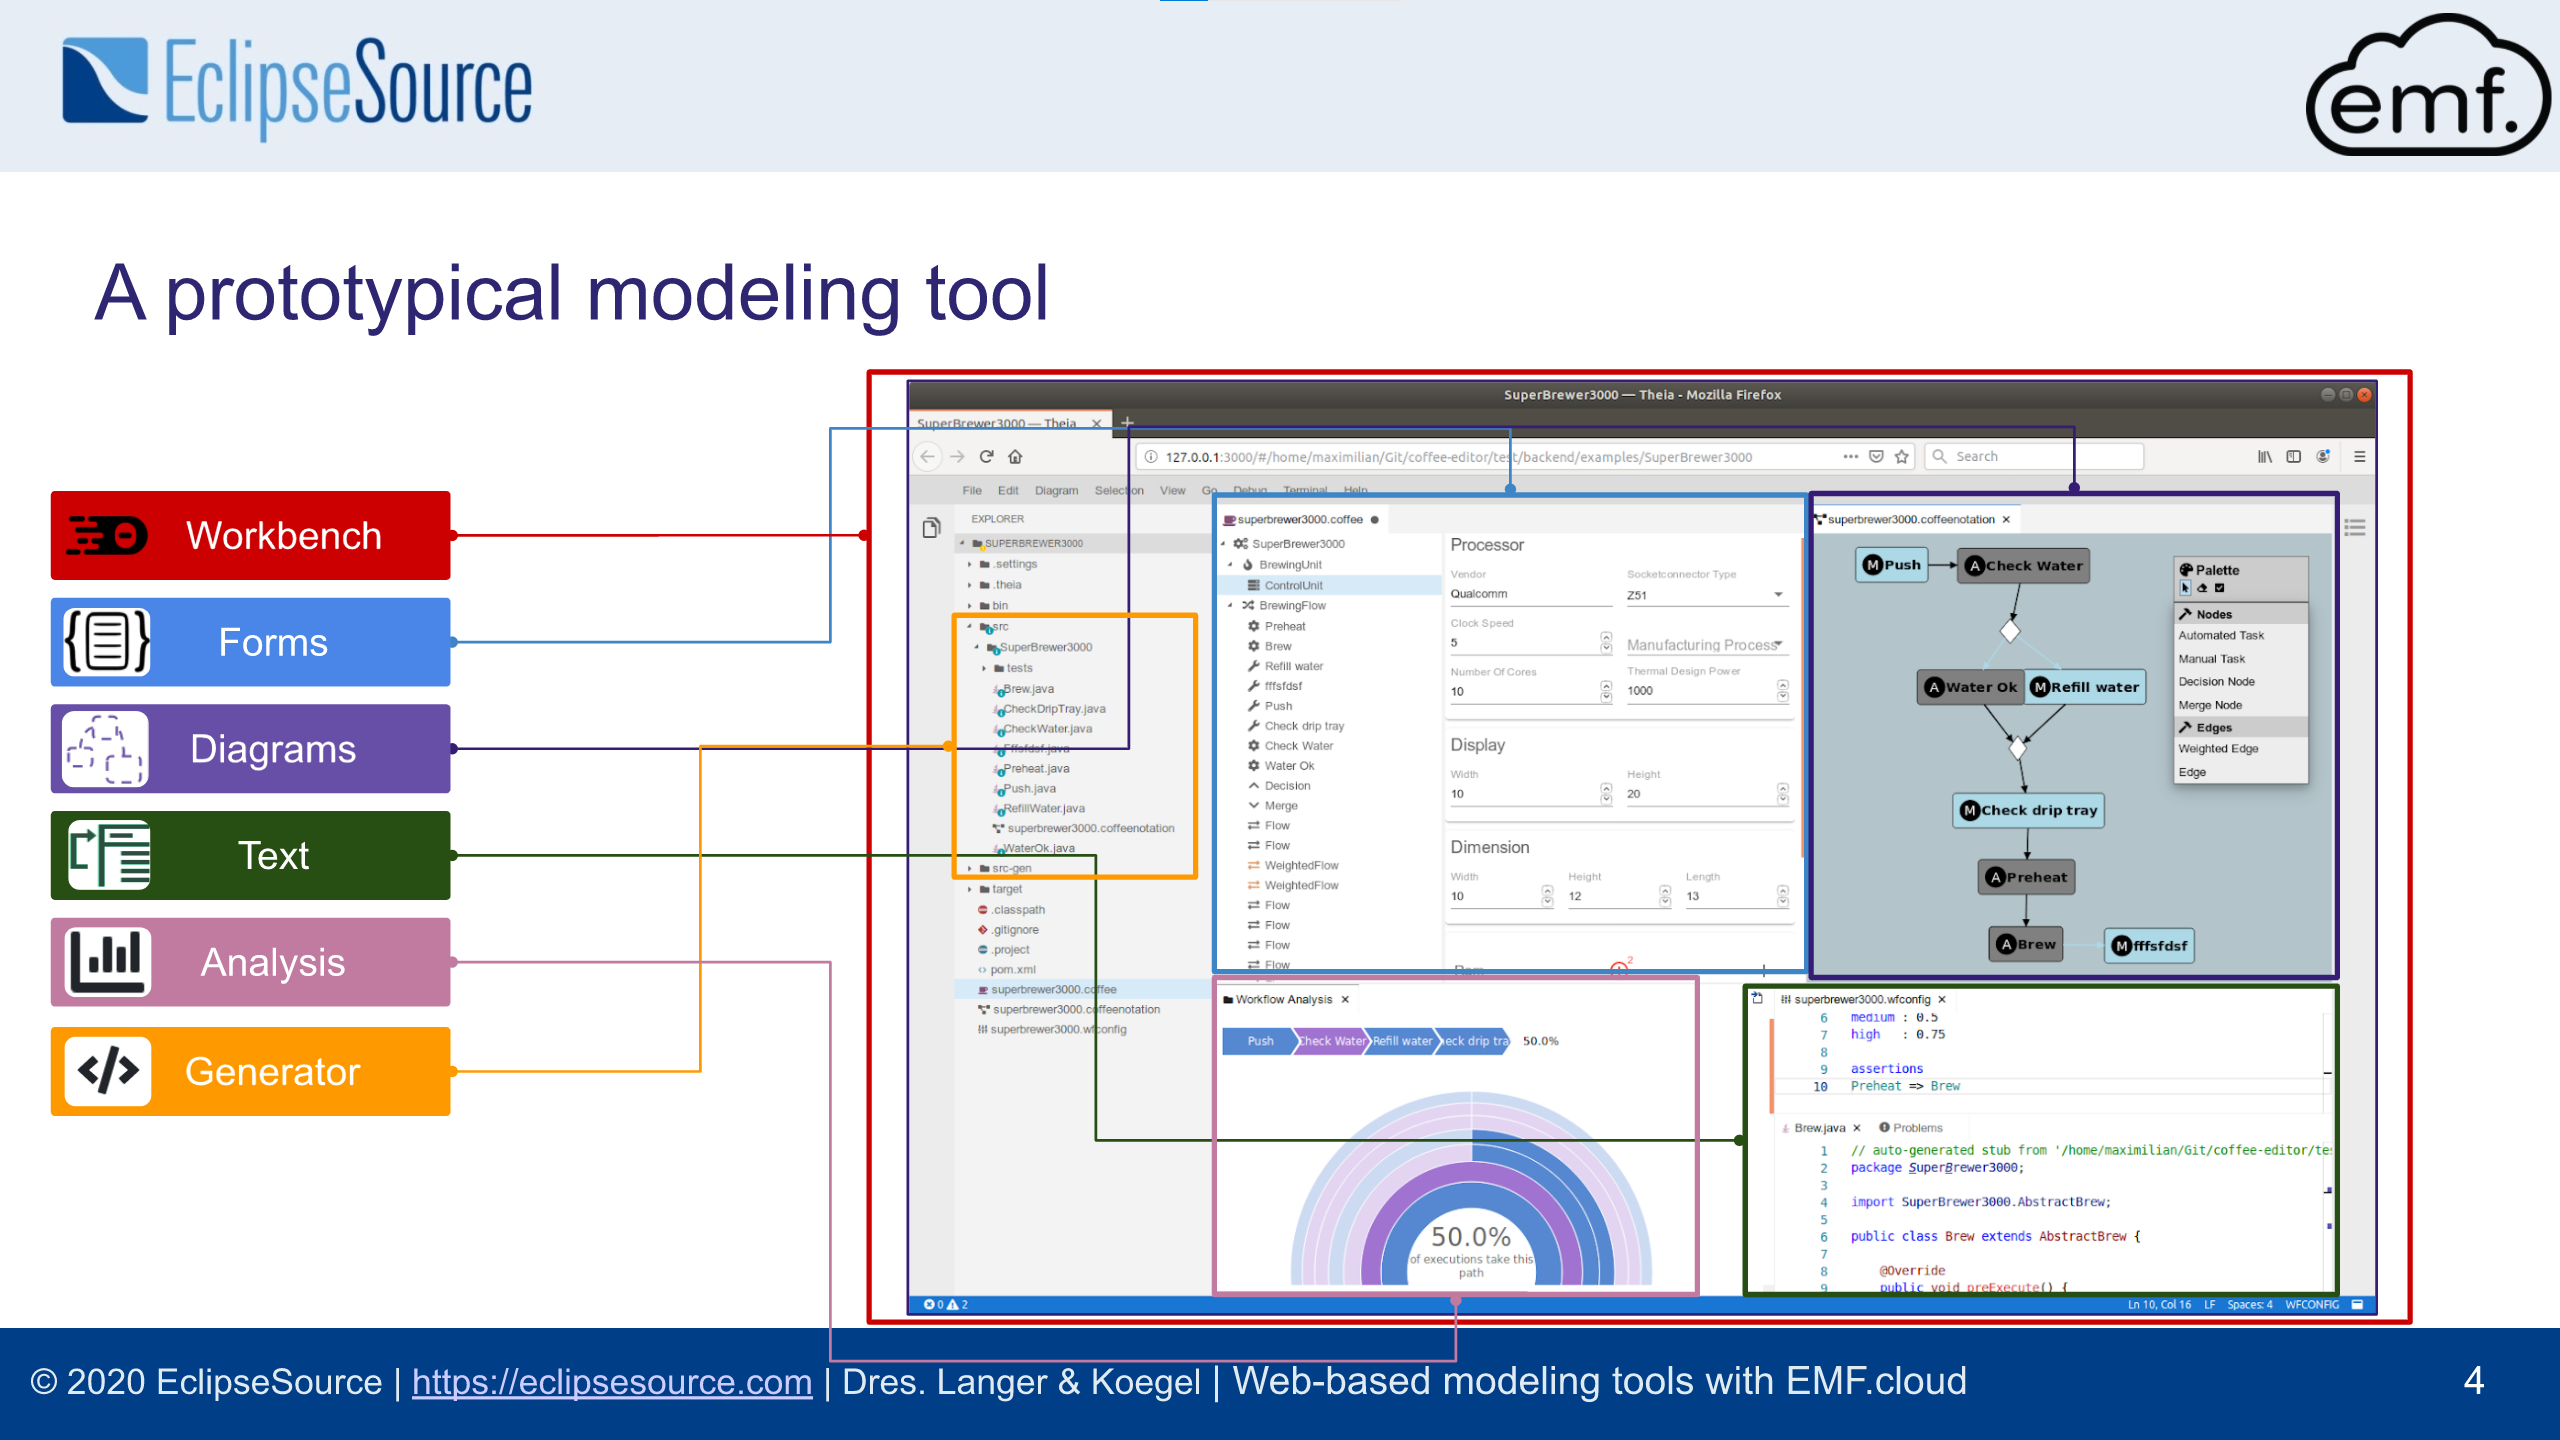
\includegraphics[width=\textwidth]{figures/coffee-maker-example}
  \caption[Coffee Editor IDE Overview]{An overview of the Coffee Editor IDE components.\cite[p.~4]{philiplangerWebbasedModelingTools2020}}\label{fig:coffee-editor-overview}
\end{figure}

\paragraph*{Intended use}
The main purpose is to show how existing editor extension components (\cref{sec:extension-components}) can be used in a real example.
This is not intended to be used by any users.

\paragraph*{Architecture}
Based on Theia with Theia Extensions and a java binary in the backend for ``analysis''\footnote{It does no analysis, it is just a proof-of-concept that sends data and views in in a graph in Theia.}.
The different editors (graphical, form, tree, textual DSL) all communicate to a shared Model Server (\cref{sec:model-server}).
This is shown in \cref{fig:coffee-maker-model-server}.
How the \gls{GLSP} and \gls{LSP} frontend components get their view of the model is by talking through the Theia extension, to a \emph{Connector} in the extension, which then talks to a \gls{GLSP}/\gls{LSP} server.
This server talks to the shared Model Server (see \cref{sec:model-server}) process. This is shown in \cref{fig:coffee-example-servers}.

\begin{figure}[!htb] 
  \centering
  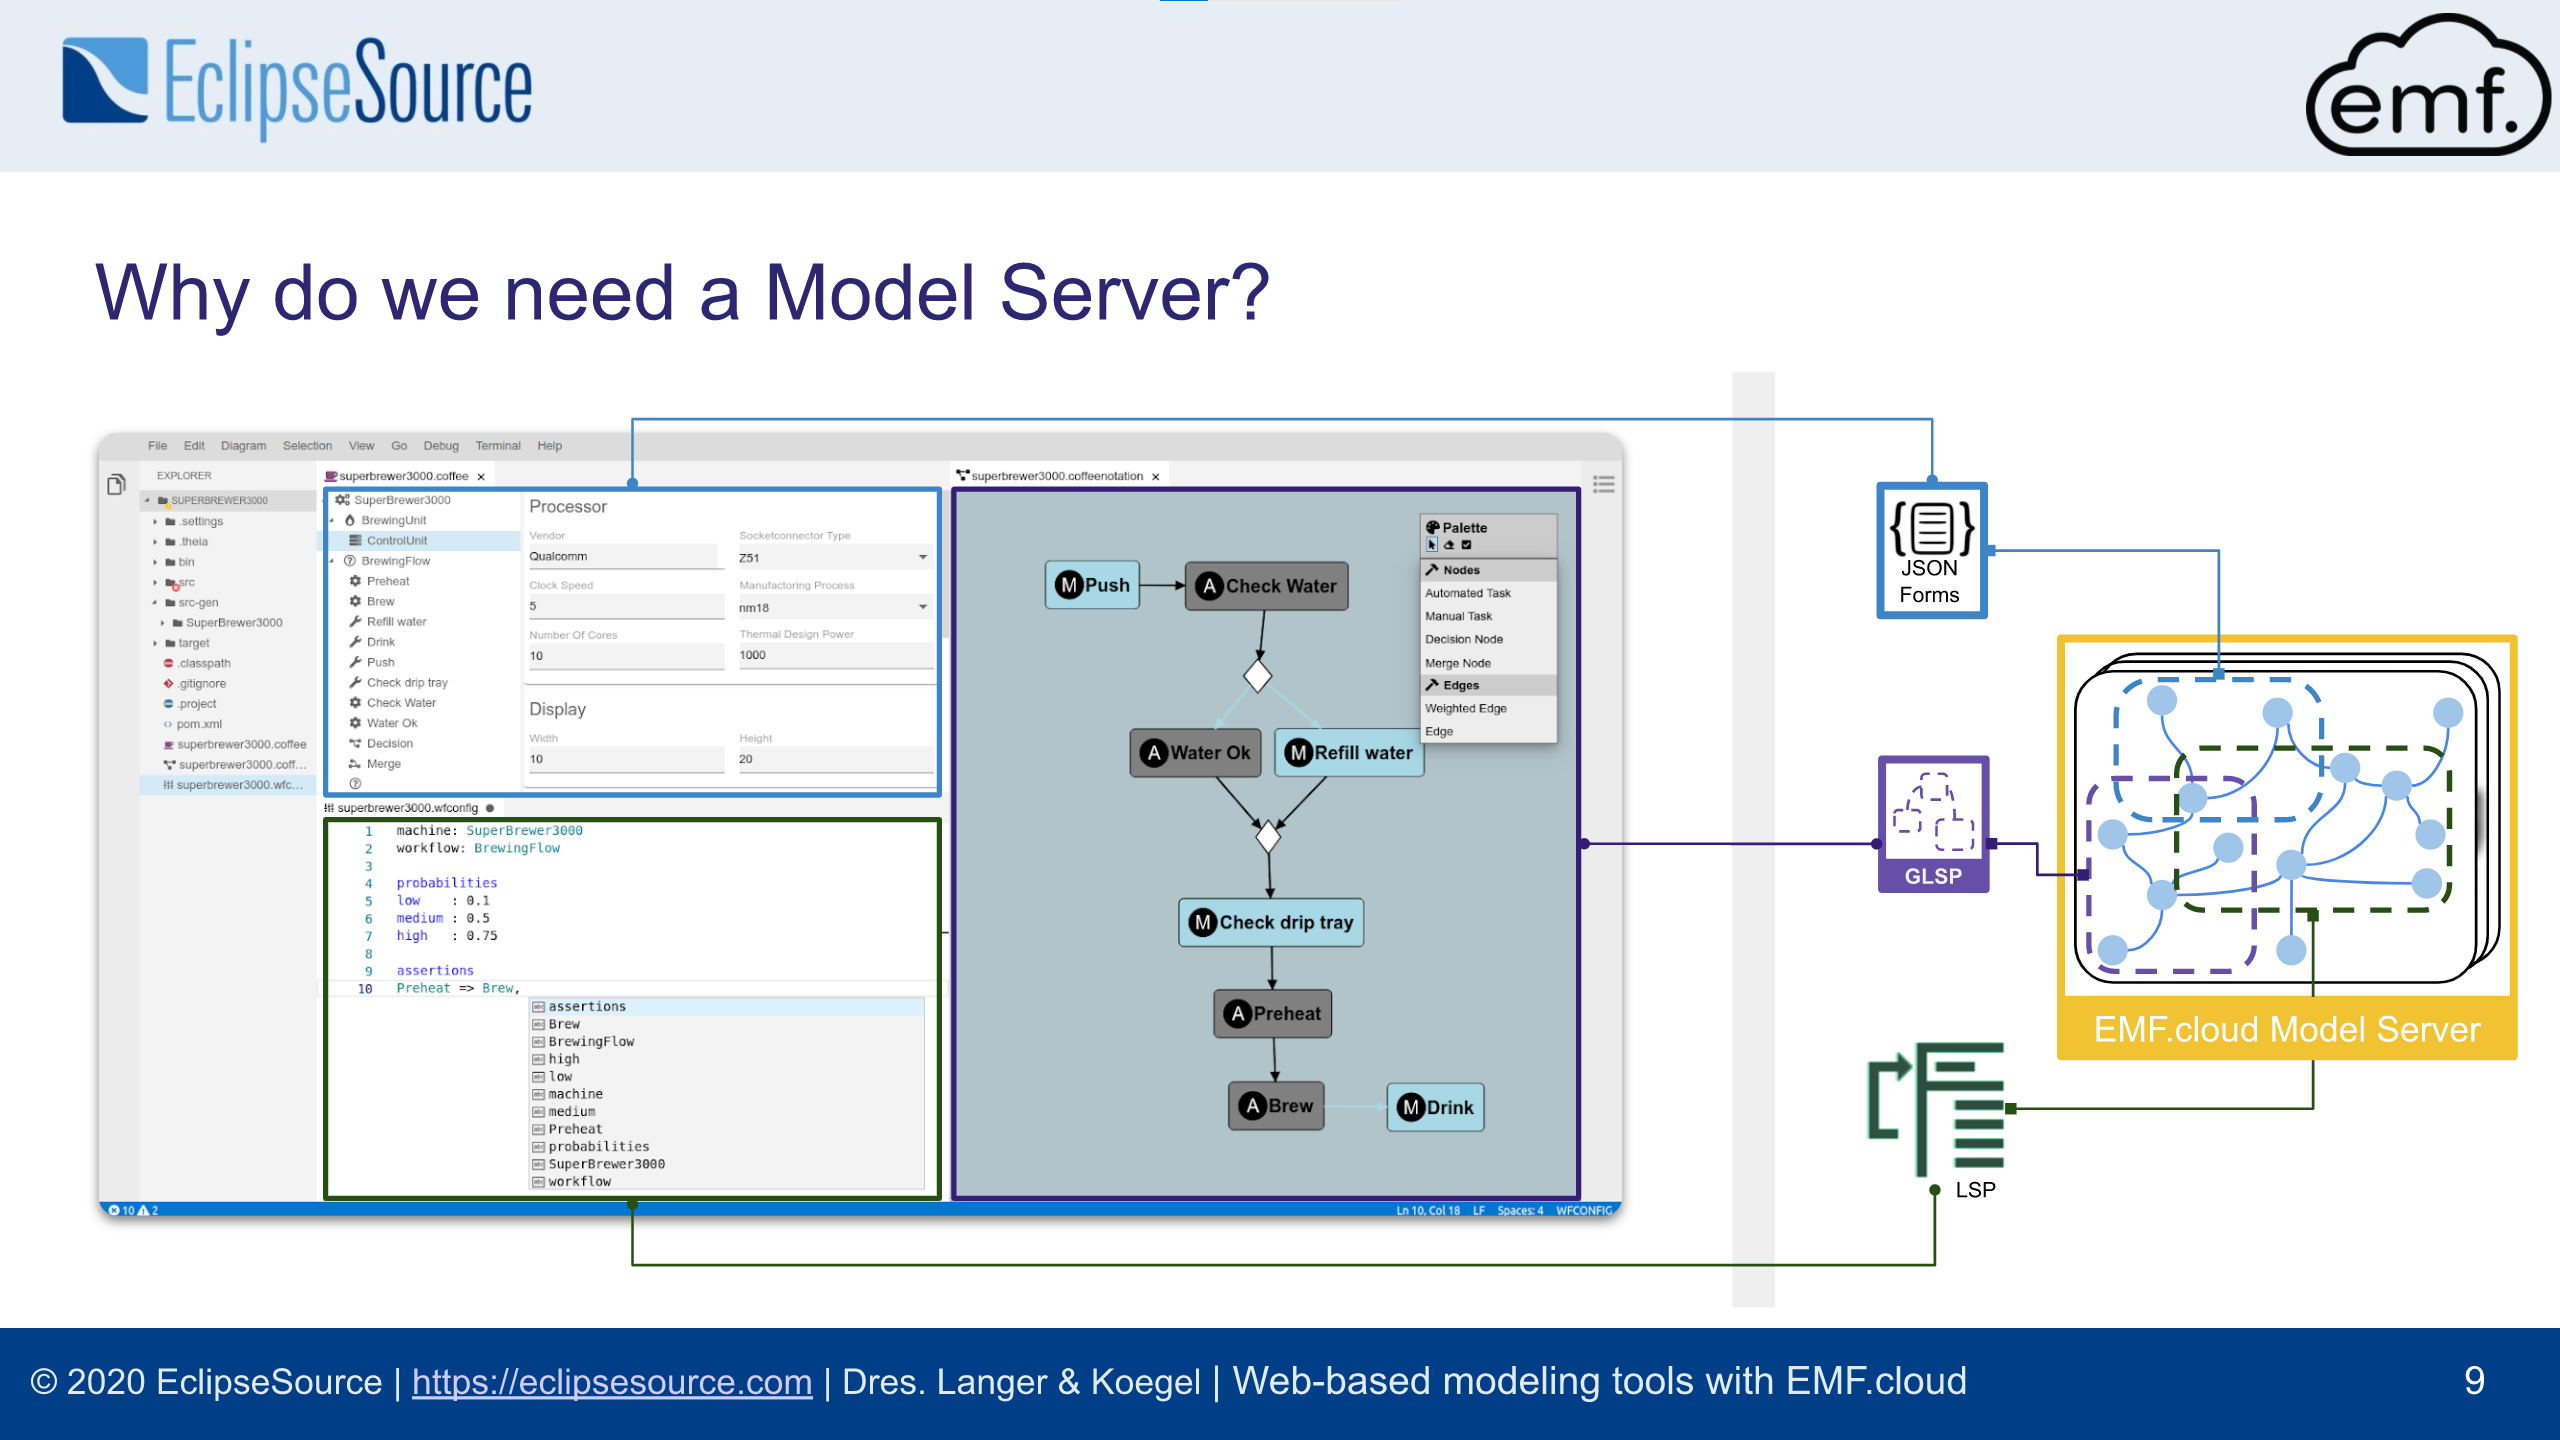
\includegraphics[width=\textwidth]{figures/coffee-maker-architecture.png}
  \caption[Coffee Editor IDE Model Server]{The Coffee Editor uses a Model Server to coordinate the different editors.~\cite[p.~9]{philiplangerWebbasedModelingTools2020}}\label{fig:coffee-maker-model-server}
\end{figure}

\begin{figure}[!htb]
    \centering
    \begin{subfigure}[b]{.45\textwidth}
        \centering
        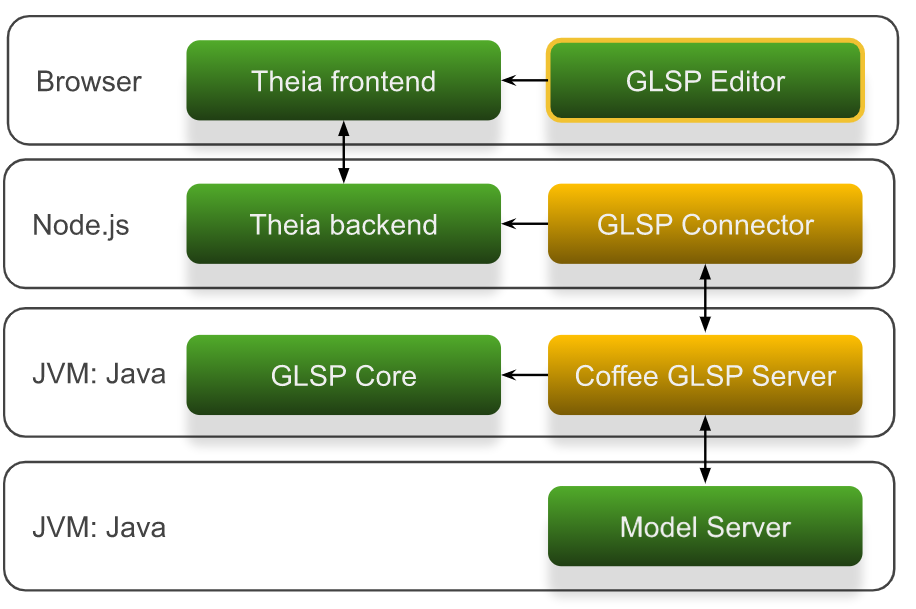
\includegraphics[width=\textwidth]{figures/coffee-maker-glsp}
        \caption{\Gls{GLSP} Editor talks indirectly to the Model Server.~\cite[p.~17]{philiplangerWebbasedModelingTools2020}}\label{sfig:coffee-example-glsp}
    \end{subfigure}
    \hfill
    \begin{subfigure}[b]{.45\textwidth}
        \centering
        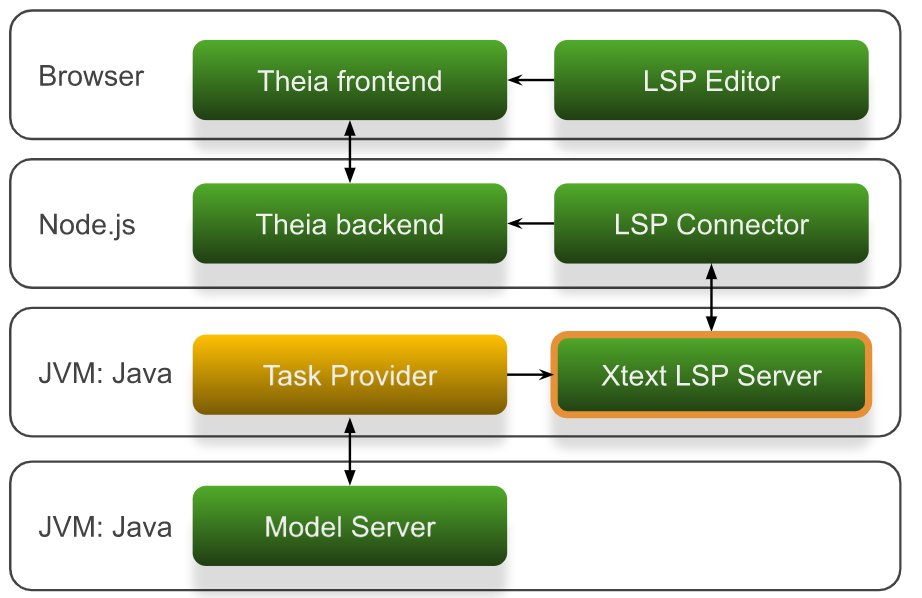
\includegraphics[width=\textwidth]{figures/coffee-maker-Xtext-LSP}
        \caption{\Gls{LSP} Editor talks indirectly to the Model Server.~\cite[p.~23]{philiplangerWebbasedModelingTools2020}}\label{sfig:coffee-example-lsp}
    \end{subfigure}
    \caption{How editors in the Coffee Editor IDE are synchronizing their model data by sharing a Model Server.}\label{fig:coffee-example-servers}
\end{figure}


\subsection{Editor Extension Mechanisms}\label{sec:extension-mechanisms}

This section will describe the extension mechanisms available for the editors in \cref{sec:editors}.

\subsubsection{VSCode Extension}\label{sec:vscode-extension}

\paragraph*{Description}
\Gls{VSCode} extensions are bundles of javascript code and resources in the \texttt{.vsix} file format.
The extensions use a \texttt{package.json} file as a \emph{manifest}, informing VSCode of the \emph{contribution points} used. 
The manifest also indicates \texttt{activation events}, which is \textit{when} an extension will be loaded (they are deactivated by default).~\cite{microsoftExtensionAnatomy2020}
The contribution points can be commands, configuration options, programming language support, debuggers, custom editors etc..~\cite{microsoftContributionPoints2020}
An extension can also contribute views to the VSCode user interface, called the \emph{workbench}, shown in \cref{fig:vscode-workbench-extension}.~\cite{microsoftExtendingWorkbench2020}
The extensions have a main entry point which is called by VSCode in a separate \gls{Nodejs} process called the \emph{Extension host}.~\cite{microsoftExtensionHost2020}
This process isolation improves the stability of VSCode in the case of crashes and hangs in an extension's code.\cite{microsoftExtensionsCapabilitiesOverview2020}

\begin{figure}[htbp]
  \centering
  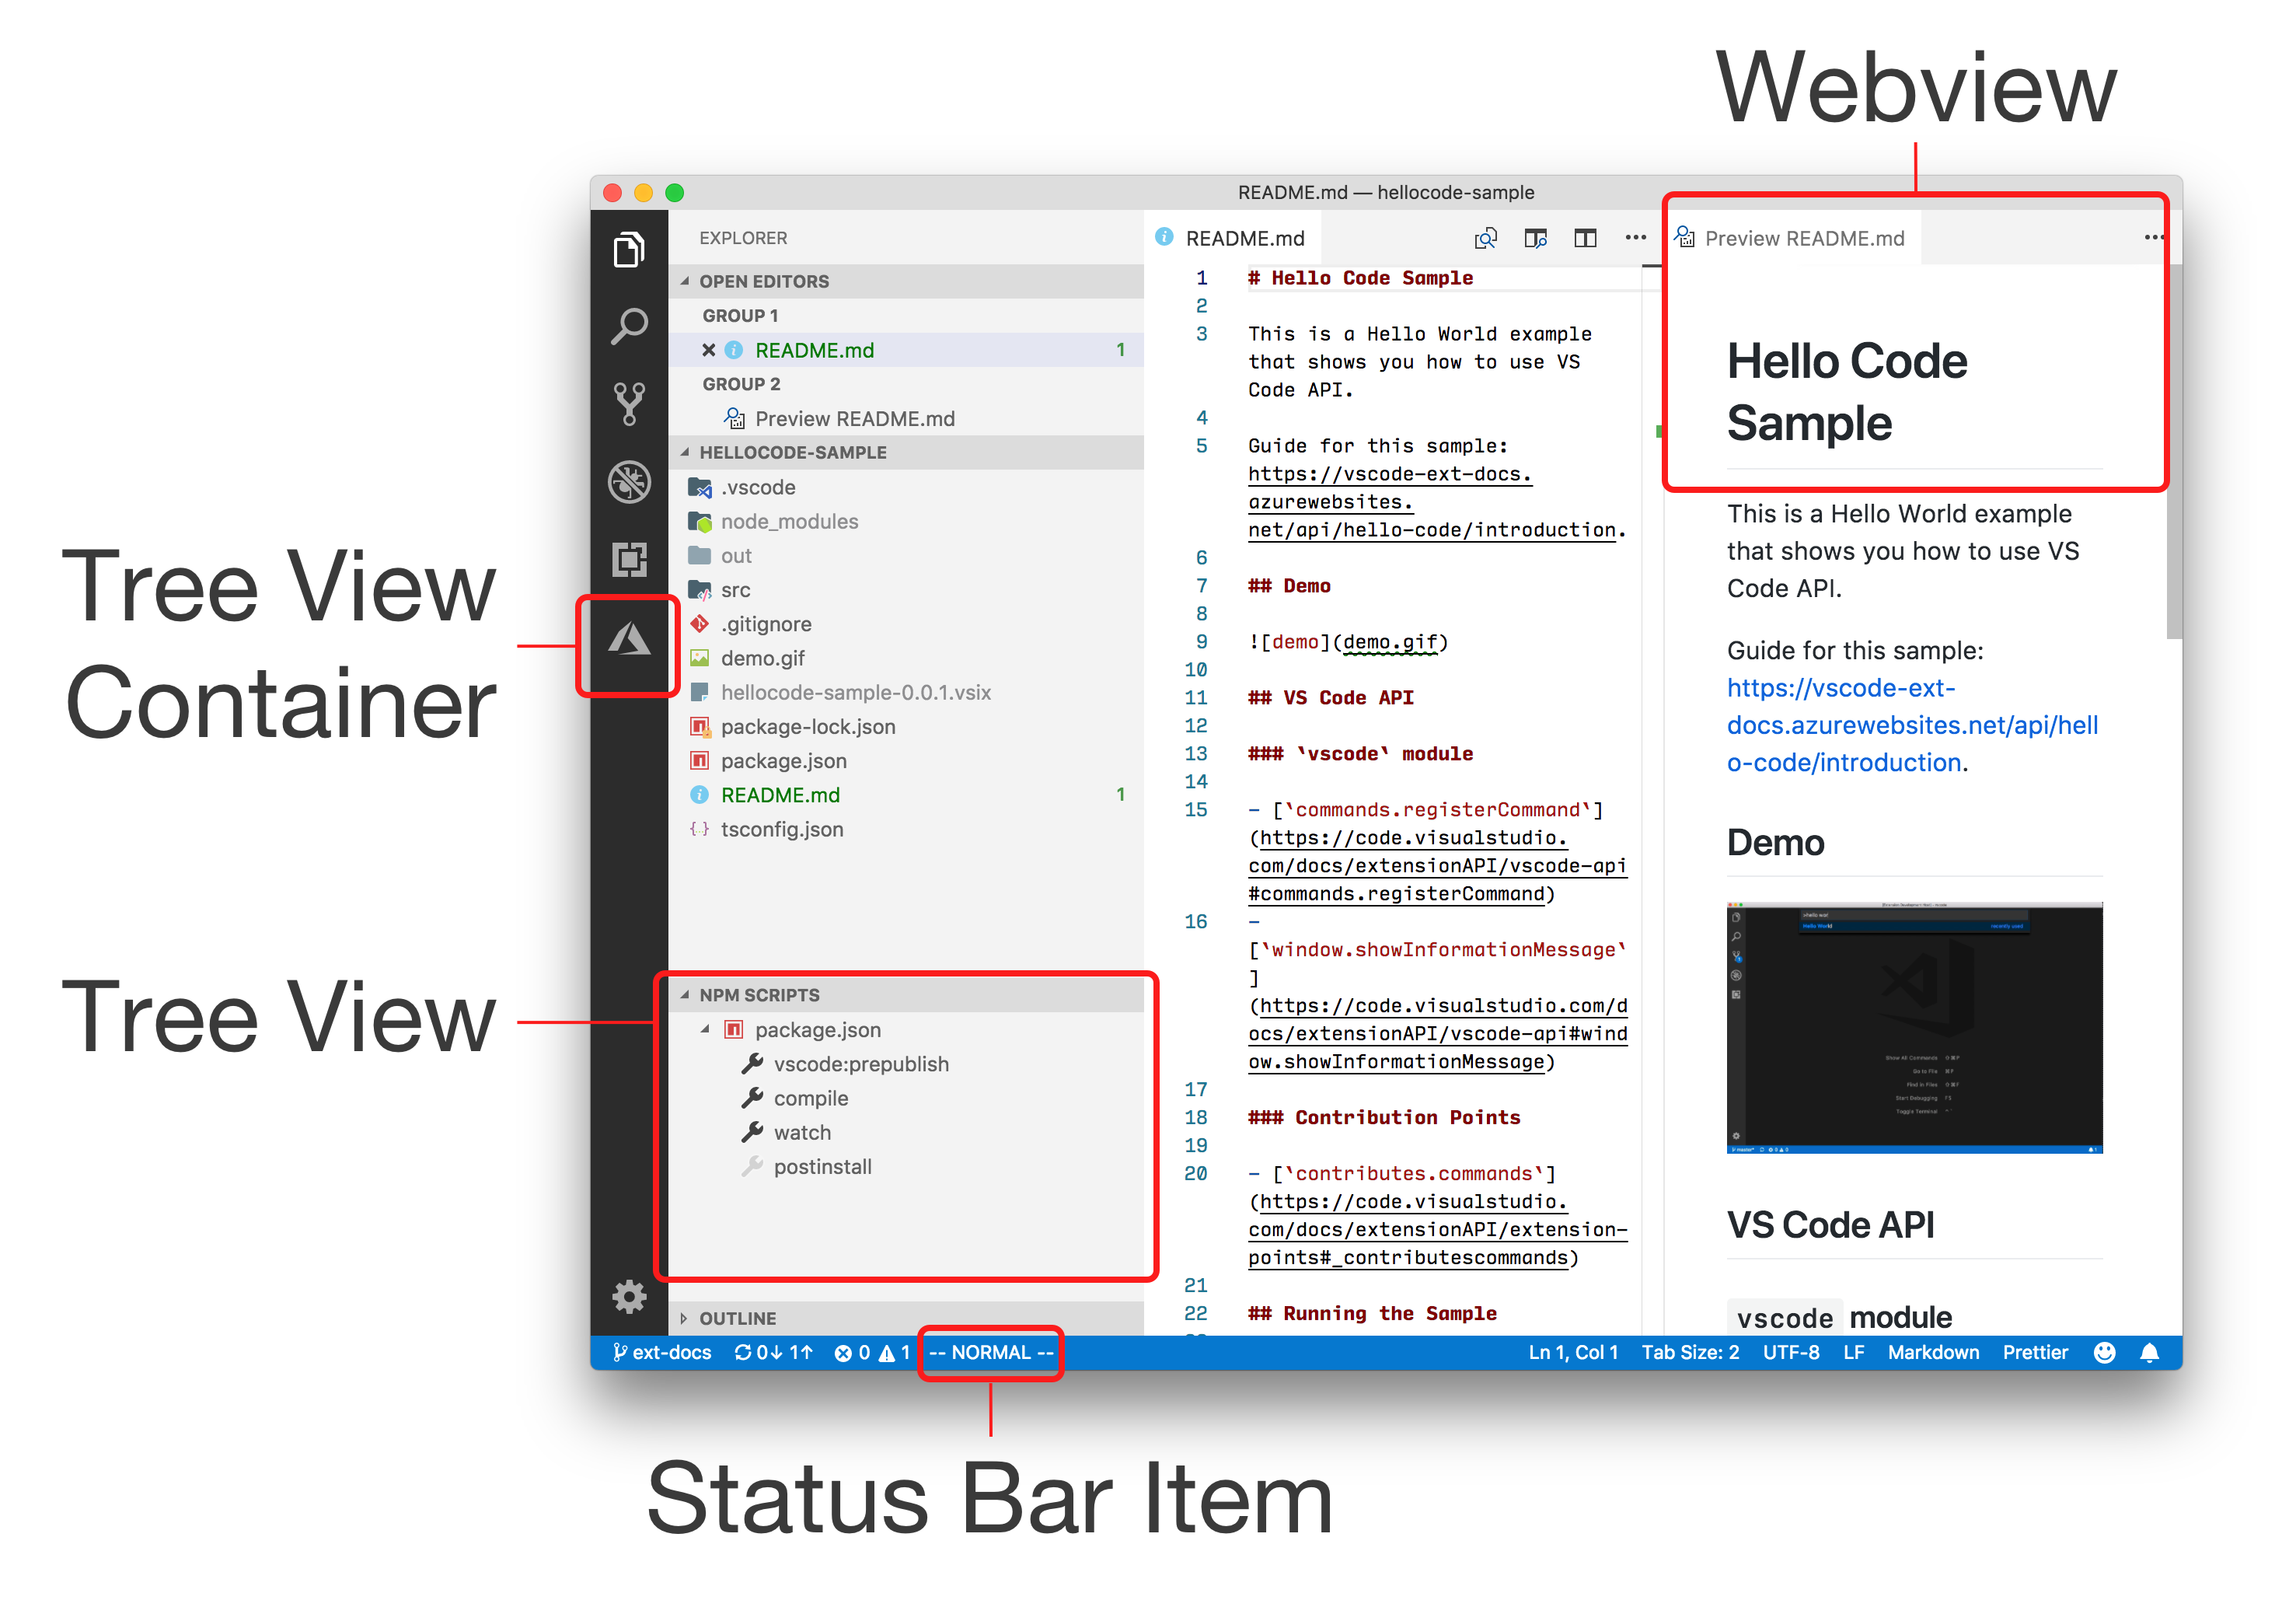
\includegraphics[width=.5\textwidth]{figures/vscode-workbench-contribution.png}
  \caption[VSCode Workbench Extension]{VSCode extensions can extend the different parts of the \emph{workbench}.~\cite{microsoftExtendingWorkbench2020}}\label{fig:vscode-workbench-extension}
\end{figure}

\paragraph*{Restrictions}
Extensions are not allowed to alter the VSCode user interface directly.~\cite{microsoftExtensionsCapabilitiesOverview2020}
All changes must be done via the provided \acrshortpl{API}.
If one wants to create custom HTML elements, the \emph{WebView} \acrshort{API} should be used.
This allows displaying HTML and running javascript.
However, this WebView is also limited: it must communicate with VSCode using \gls{JSON} messages, and relies on VSCode to save its state by handing sending it over.~\cite{microsoftWebviewAPI2020}


% Who can use it
% How is it structured?
% What can it do?
% How is it distributed?

\subsubsection{Theia Plugin}\label{sec:theia-plugin}

\paragraph*{Description} \Gls{Theia} \emph{plugins} are exactly the same as VSCode extensions in \cref{sec:vscode-extension}.
A Theia Plugin does not need to separate frontend and backend code.
The VSCode \acrshortpl{API} are transparently separated between the frontend and backend using \gls{JSON-RPC}.~\cite{paulmarechalTheiaPluginImplementation2020}
The support for VSCode extensions was added to Theia so \gls{Che} (which uses Theia) could allow users to install extensions without impacting the stability of the \acrshort{IDE}.~\cite{helmingEclipseTheiaExtensions2019}
A \emph{Theia Extension} could crash and bring down the entire editor, in contrast to a \emph{Theia Plugin} (VSCode extension) which would only display a warning.
Because of licensing issues\footnote{Only Microsoft products can use the marketplace.~\cite{svenefftingeOpenVSX2020}} with Microsoft and its VSCode extension marketplace, all Theia Plugins are hosted on a independent marketplace called \emph{OpenVSX}\footnote{\href{https://open-vsx.org}{https://open-vsx.org}} instead.~\cite{svenefftingeOpenVSX2020}

\paragraph*{Creating a Theia Plugin}
A developer can follow the same tutorials that VSCode Extensions provide, and use the same \acrshortpl{API}.
There is no need to do anything special for Theia to run a VSCode Extension.
However, only a subset of the \acrshortpl{API} are \emph{implemented} yet in Theia.
This is because of time constraints, not policy; more \acrshortpl{API} are supported as developers find time.

\paragraph*{Supported VSCode APIs}
A list of supported \acrshortpl{API} can be found at \href{https://che-incubator.github.io/vscode-theia-comparator/status.html}{https://che-incubator.github.io/vscode-theia-comparator/status.html}.
Most notably for this thesis, is that the \texttt{registerCustomEditorProvider}, \texttt{CustomEditorProvider} and \texttt{createWebviewPanel}\footnote{However, this merge says Theia should support it \href{https://github.com/eclipse-theia/theia/pull/3484}{https://github.com/eclipse-theia/theia/pull/3484}.} are not supported yet.
(Progress for Custom editors can be followed in \href{https://github.com/eclipse-theia/theia/issues/6636}{https://github.com/eclipse-theia/theia/issues/6636}).

\paragraph*{Installing a Theia Plugin}
Either search for the plugin inside the plugin browser provided by \gls{Theia},
or drag-and-drop a \texttt{.vsix} file into the extension browser.
Theia will only search for plugins on OpenVSX, not the Visual Studio Marketplace.

% Who can use it
% How is it structured?
% What can it do?
% How is it distributed?


\subsubsection{Theia Extension}\label{sec:theia-extension}

\paragraph*{Description}
\Gls{Theia} Extensions are the building blocks of Theia.
They are loaded at launch time, not run time.
Dependency injection is used to discover and load extensions.
Extensions were the original mechanism added to Theia for customizing its behavior.
They are allowed full access to Theia, and can do anything\footnote{Within the scope of browsers and \gls{Nodejs}.}.~\cite{helmingEclipseTheiaExtensions2019,helmingEclipseTheiaIDE2019a}
All the main features of Theia are provided using Theia Extensions.

\paragraph*{Installing an extension}
To install a Theia Extension, a developer has to compile Theia itself.
The extension must be available as a package, e.g.\ on \gls{NPM} or as a local folder, and added to the \texttt{package.json} as a dependency.~\cite{helmingHowAddExtensions2019}
For an \gls{NPM} package, the extension's \texttt{package.json} should contain \texttt{``theia-extension''} in the \texttt{keywords}.~\cite{typefoxAuthoringTheiaExtensions}

% Who can use it
% How is it structured?
% What can it do?
% How is it distributed?

% Eclipse plugin? Probably not


% Architectures? Eclipse Plugin, Theia Extension

\section{Prototypes}

Prototypes are used to answer some of the research sub-questions.
First, one or more questions are selected for a prototype.
Then a design document is created, which details goals and architecture of the prototype.
Next, the implementation is done.
Finally, the implementation is executed and evaluated.


This thesis has a total of two prototypes.
The first, \emph{prototype 1}, aims to answer \cref{rq:22}.
The second, \emph{prototype 2}, aims to answer \cref{rq:23}, \cref{rq:24}, \cref{rq:25} and \cref{rq:26}.


\subsection{Prototype 1}

This prototype tries to answer \cref{rq:22}:
\begin{displayquote}
  How can java applications be used in a VSCode extension?
\end{displayquote}


\subsubsection{Requirements}

\begin{itemize}
  \item Develop using VSCode extension \acrshort{API} (see \cref{sec:vscode-extension}). No dependencies to Theia.
  \item Embed an executable java \texttt{.jar} file into the extension
  \item Install in both VSCode and Theia (Gitpod)
  \item Execute the \texttt{.jar} using a pre-installed java runtime
  \item Communicate bi-directionally with the started java process from the extension backend, using \texttt{standard input/output (stdio)} and over a TCP socket. (Only Theia has the concept of backend and frontend)
\end{itemize}

The \textit{design document} used for implementation is added in \cref{app:prototype-1-design-doc}.

\subsubsection{Implementation}

\paragraph*{Project creation}
An extension project was created using a project generator, \emph{yeoman}, and a project template called \emph{generator-code}.~\cite{microsoftYourFirstExtension2020}


\paragraph*{First step}
To test if an extension could call \emph{any} executable binary file at all, the first goal was to run the linux \texttt{ls} command.
By using the \gls{Nodejs} standard library function \texttt{child\_process.spawn}, and printing the outputs to a \gls{VSCode} information popup, this test was created.
This intermediate result was a success, and a popup with folder contents was shown, as illustrated in \cref{fig:prototype-1-ls}.

\begin{figure}[htbp]  % order of priority: h here, t top, b bottom, p page
  \centering
  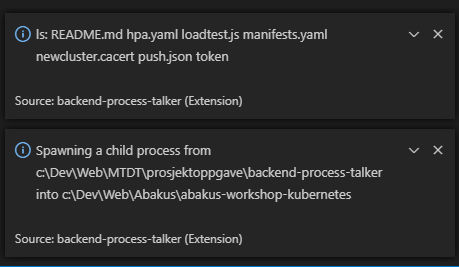
\includegraphics[width=.5\textwidth]{figures/vscode-extension-child_process-ls}
  \caption[VSCode Communicates with a Binary Executable]{VSCode executes a binary executable and displays its output.}\label{fig:prototype-1-ls}
\end{figure}

\paragraph*{Preparing a java jar file}
Next, a \texttt{.jar} file was creted from a java project.
This project was a separate one from the VSCode extension.
It would create an executable \texttt{.jar} which would echo back any text sent to its \emph{standard input}. The executable could also listen to a TCP port on \emph{localhost}, and echo back there.
For the \texttt{.jar} to be executable, the \texttt{main} method was registered in the \texttt{META-INF} file as the entry point.

\paragraph*{Running the jar in VSCode}
The code to execute \texttt{ls} was modified to run the \texttt{.jar} instead.
The \texttt{.jar} was placed in a (arbitrarily) named folder \emph{lib} in the VSCode extension project root.
To get the file path to the \texttt{.jar}, a \gls{VSCode} \acrshort{API} was used.
A code snipped illustrating this is shown in \cref{lst:prototype1-jar}.
Triggering the execution of the file was done using a \gls{VSCode} \emph{command} defined in the prototype, named \texttt{Hello World}.
Text was sent using standard input/output (\texttt{stdin, stdout}).
(Another version of the extension was also tried, sending data over TCP to a predefined port on \emph{localhost} (the same machine).)

\lstinputlisting[
    caption={Typescript code to run a java \texttt{.jar} in \gls{Nodejs}.},
    label=lst:prototype1-jar,
    language=Typescript
]{listings/run_jar_from_vscode.ts}

\paragraph*{Bundling the extension}
The last step is to create a bundle.
It is crucial that the bundle has the \texttt{.jar} file inside it, otherwise the extension would fail to run it, and this prototype would have a major problem.
A tool called \texttt{vsce} was installed and used.
This tool created a \texttt{.vsix} file, which is the extension installer.
Theia as VSCode needs this file, as it contains the prototype's code.
The \texttt{vsce} tool has a \texttt{ls} command, which shows all the files it will put into the bundle.
This command was executed, and the \texttt{.jar} file \emph{was} listed.

\paragraph*{Installing the extension}
Installation in VSCode is done by pressing \texttt{ctrl + shift + P} (on windows) and typing \texttt{>extensions: Install from vsix}, and then browsing to the file.
Installation in Theia is done by opening the \emph{Extensions} panel, and dragging the \texttt{.vsix} file into it.
The Theia instance used was in Gitpod with the \emph{Theia source code} workspace open\footnote{\href{https://gitpod.io/\#https://github.com/eclipse-theia/theia}{https://gitpod.io/\#https://github.com/eclipse-theia/theia}, requires login.}

\paragraph*{Activating the extension}
After installation, the Theia \emph{Commands} prompt was opened by pressing \texttt{F1} on the keyboard.
Then \texttt{Hello World} was entered, which is the name of the extension's \emph{command}.
Theia proceeded to show the outputs of the \texttt{.jar} file in a information popup.

\begin{figure}[htbp]  % order of priority: h here, t top, b bottom, p page
  \centering
  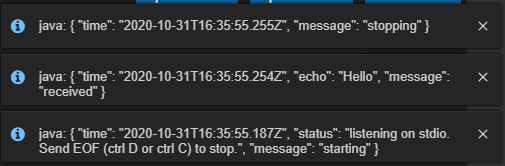
\includegraphics[width=.5\textwidth]{figures/theia-talks-to-jar-in-vscode-extension-via-stdio}
  \caption[Theia Executes a Bundled Jar File]{Theia is showing information popup windows that contain the outputs of executing a \texttt{.jar} file.}\label{fig:prototype1-theia-jar}
\end{figure}


\subsubsection{Results}
Because the extension resulted in a \texttt{.vsix} file with a \texttt{.jar} inside, and was installed and used in Theia successfully, the first prototype was a success.

The answer to \cref{rq:22} is:
\begin{displayquote}
  \emph{by bundling the java application as an executable \texttt{.jar}, and then starting it as a child process with the \gls{Nodejs} \acrshort{API} \texttt{child\_process.spawn}. Communication can be done from the Theia backend (or VSCode) over standard input/output or a network socket to a port on localhost.}
\end{displayquote}
  
This is based on the assumption that the \emph{host operating system has a java runtime installed and available on the path}.
However, this runtime \textit{could} be bundled itself.

Note that the Theia \emph{frontend} did \emph{not} communicate directly with the child process.
All communication was done by the backend and relayed to the frontend over \gls{JSON-RPC}.
\subsection{Prototype 2}

This prototype tries to answer \cref{rq:23}, \cref{rq:24}, \cref{rq:25} and \cref{rq:26}:
\begin{displayquote}
  How should the editor cooperate with multiple other tools that change the same underlying model?\\
  What data is required for displaying a model as a tree?\\
  How can a tree editor component be generic enough to support arbitrary user actions?\\
  How can the user interface know the model well enough so the user is constrained from creating invalid Ecore trees?
\end{displayquote}

\subsubsection{Requirements}

\paragraph*{Cooperation (\cref{rq:23})}
Cooperation in \cref{rq:23} could possibly be solved by channeling any model edits through a Model Server, and listening to this server for change notifications. An example of this was seen in \cref{sec:coffee-ide} with the \emph{Coffee Editor} reference implementation for \gls{GLSP} (\cref{sfig:coffee-example-glsp}).

\paragraph*{Tree model (\cref{rq:24})}
By displaying an example tree, the required data will be evident as the view is implemented.

\paragraph*{Generic actions (\cref{rq:25})}
By supporting actions through buttons in the user interface, but not hardcoding their clicks to trigger an action, they can be generic.
This means a click must only notify something that an \emph{intent} to trigger action \texttt{XYZ} has happened.
Implementing a skeleton for this would show what data is required for generic actions.

\paragraph*{Constrain tree for validity (\cref{rq:26})}
This is relevant especially for drag-and-drop, where a user should not be able to drop a node onto an ``incorrect'' parent.
Due to time constraints, drag-and-drop will not be implemented now.
But the supporting data structure could be sketched out, based on the previous data structures for the Tree model in \cref{rq:24}.

\paragraph*{Here is the list of identified requirements for this prototype:}

\begin{itemize}
  \item Develop using VSCode extension \acrshort{API} (see \cref{sec:vscode-extension}). No dependencies to Theia.
  \item Visualize a tree structure in the editor, based on a object structure (e.g. \gls{JSON}).
  \item Show labels and icons for nodes in the tree. Labels will be from node \emph{type}, labels from node data.
  \item Add and remove nodes in the tree from user interaction.
  \item Property sheet editor that is synchronized with tree selection.
  \item Visualize both an Ecore meta-model and model instance.
  \item Use EMF.Cloud Model Server (\cref{sec:model-server}) to get the model. Do not read the \texttt{.ecore} file from disk in the extension.
  \item Automatically update the views when the underlying model changes (push not poll)
\end{itemize}

The \textit{design document} used for implementation is added in \cref{app:prototype-2-design-doc}.

\subsubsection{Implementation}

\paragraph*{Setting up the project}
Similar to prototype 1, a new \gls{VSCode} Extension project was created.
A \emph{standalone} version of the EMF.Cloud Model Server (\cref{sec:model-server}) was downloaded\footnote{Snapshot builds are provided at sonatype: \href{https://oss.sonatype.org/content/repositories/snapshots/org/eclipse/emfcloud/modelserver/org.eclipse.emfcloud.modelserver.example/0.7.0-SNAPSHOT/}{https://oss.sonatype.org/content/repositories/snapshots/ org/eclipse/emfcloud/modelserver/org.eclipse.emfcloud.modelserver.example/0.7.0-SNAPSHOT/}.}
Unlike Coffee Editor IDE, this implementation does not use Theia Tree Editor (\cref{sec:theia-tree-editor}), because of its incompatibility with \gls{VSCode}.
A minimal, ``homemade'' solution was made instead, with CSS, HTML lists (\texttt{ol} and \texttt{li}) and some javascript.

\paragraph*{Connecting to VSCode APIs}
The editor had to use the \texttt{WebView} \acrshort{API}, being a non-text editor.
The javascript and CSS for a WebView exists in a separate folder without access to the rest of the extension code.
This is based on an official Microsoft tutorial called \emph{PawDraw}\footnote{\href{https://github.com/microsoft/vscode-extension-samples/tree/master/custom-editor-sample}{https://github.com/microsoft/vscode-extension-samples/tree/master/custom-editor-sample}.}.

The other piece of the puzzle was a \texttt{CustomDocument} and \texttt{CustomEditorProvider}.
These act as the glue between the \texttt{WebView}, VSCode and the extension.
Saving and file operations run through these \acrshortpl{API}.
Most of the handlers on \texttt{CustomEditorProvider} were left unimplemented, as only \texttt{resolveCustomEditor} was crucial.
This is the function that configures the \texttt{WebView} for the extension, providing it the tree editor HTML, javascript and CSS etc..

\paragraph*{The Tree Editor WebView}
Inside the \texttt{WebView} lives the actual editor user interface.
It has security restrictions when it comes to where resources (images etc.) can be loaded from.
To test a method for arbitrary icons, an image encoding called \emph{data-uri} was used.
It simply encodes the raw image to a Base64 string and prepends some metadata.
The result is one long string for one image.
A protocol could pass these images for tree node icons instead of referring to file paths.
A data structure mapped node types to an icon string, as seen in \cref{lst:prototype2-default-icons}.

\lstinputlisting[
    caption={Javascript code from the WebView to map icon graphics to tree node types.},
    label=lst:prototype2-default-icons,
    language=JavaScript
]{listings/default-icons.js}

To get the data for tree nodes, a sample data structure was created (see \cref{lst:prototype2-node-tree} for the data).
No real \gls{emf} or \gls{XMI} data was read in yet.
The fields in the structure were evolved alongside the tree view, adding or restructuring properties when issues arose.
A \texttt{name} was deemed essential for every node, and moved outside of the \texttt{properties}.
For determining the \emph{node types}, the \gls{Ecore} class name was used as the type.
(It is uncertain how this works with generics or inheritance, but I assume the type parameters and children could be mapped into the type value, e.g. by appending them).
Clicking on a node would store the node as the \emph{selected node}, and trigger an event listener (so the property sheet and action bar could update).

\lstinputlisting[
    caption={Javascript code from the WebView for a data model describing the tree nodes.},
    label=lst:prototype2-node-tree,
    language=JavaScript
]{listings/node-tree.js}

\paragraph*{Form based property editor}
A simple form was updated with the data of the selected tree node.
Changes were sent as notifications to VSCode.
These notifications only accept data that can be serialized to \gls{JSON}.
(The communication from the \texttt{WebView} to the \gls{VSCode} Extension \emph{could} possibly be made with \gls{JSON-RPC} in the future. It was not needed for now).

\paragraph*{Action bar}
An area with buttons was created to trigger arbitrary model actions, such as on-demand validation, genmodel code generation and dynamic instance creation.
The actions took their label from an action list, and every action has an \emph{id}. This is shown in \cref{lst:prototype2-action-list}.
Icons could be added in the same way, but was not done.
This abstracts actions to only id and label, and then the Tree Language Server could deal with the details of triggering the action.

\lstinputlisting[
    caption={Javascript code from the WebView to specify the available actions.},
    label=lst:prototype2-action-list,
    language=JavaScript
]{listings/available-actions.js}

A list specified which id to always show in the action bar.
Another data structure held mappings between node types and lists of actions.
This would allow different actions to be available based on the selected tree node. This is shown in \cref{lst:prototype2-action-schema}.

\lstinputlisting[
    caption={Javascript code from the WebView to specify default actions and per-node actions.},
    label=lst:prototype2-action-schema,
    language=JavaScript
]{listings/action-schema.js}


\paragraph*{Constraining the tree hierarchy}
No user manipulation of the tree was implemented, due to time constraints.
But a data structure that could identify which children are valid for a node type was specified.
This is shown in \cref{lst:prototype2-hierarchy-schema}.
The idea is to consult this mapping when deciding if a child node can be put into a specific parent node, which happens during drag-and-drop and copy-paste operation.


\lstinputlisting[
    caption={Javascript code from the WebView to specify what children a node type can have.},
    label=lst:prototype2-hierarchy-schema,
    language=JavaScript
]{listings/hierarchy-schema.js}


\paragraph*{Model Server}
The model server was only partially integrated, due to time constraints.
It was started manually, and only a single endpoint was used, which was selecting the \emph{model workspace directory}.
This is the directory where the Model Server will scan for \texttt{.ecore} and \texttt{.xmi} files.
The extension send a request to the Model Server's \gls{REST} \acrshortpl{API} with the workspace folder.
A testing command to create a new model file was also implemented.
This was a VSCode Command which prompted the user for a filename.
Then the extension would send the filename and an example EObject (serialized as \gls{JSON}) to the Model Server.
The Model Server would create a new \gls{XMI} file when receiving this request.


\subsubsection{Results}
The editor worked, but due to time constraints, some features were dropped.
Mainly user editing and model updates were not done, as well as automatic ecore-model-to-tree conversion.
A screenshot of the model is shown in \cref{fig:prototype-2-screenshot}.

\begin{figure}[htbp]
  \centering
  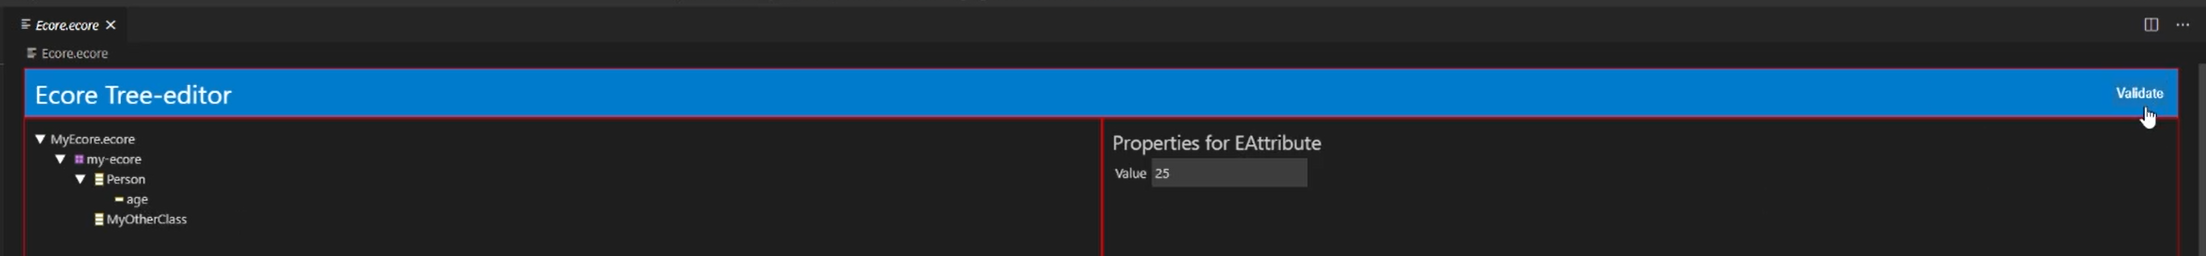
\includegraphics[width=\textwidth]{figures/prototype-2-screenshot.png}
  \caption[Prototype 2 Screenshot]{A screenshot of the prototype 2 in action. It has three parts: an action bar on the top right, a tree view on the left, and a property editor on the right.}\label{fig:prototype-2-screenshot}
\end{figure}

\paragraph*{Research questions}
The answer to \cref{rq:23} is:
\begin{displayquote}
  \emph{By reading the model data structure from a shared model server, and only editing it by sending commands to this model server.}
\end{displayquote}

The answer to \cref{rq:24} is:
\begin{displayquote}
  \emph{A nested datastructure of nodes, with labels and node types, as well as properties for each node. See \cref{lst:prototype2-node-tree} for an example.}
\end{displayquote}

The answer to \cref{rq:25} is:
\begin{displayquote}
  \emph{By only defining actions as id and label, and sending a schema of default actions and per-node actions to the frontend. Triggering an action will only send a message to the backend Tree Language Server, where this server executes any actual change. See \cref{lst:prototype2-action-list} and \cref{lst:prototype2-action-schema}} for examples.
\end{displayquote}

The answer to \cref{rq:26} is:
\begin{displayquote}
  \emph{By defining a parent-child schema based on node types, that specifies which children are allowed in a parent. See \cref{lst:prototype2-hierarchy-schema} for an example.}
\end{displayquote}
This last answer was not properly tested due to time constraints.

\section{Tree Editor}\label{sec:result-tree-editor}

This section will present the findings for a \emph{Tree Editor}.

\subsection{Functional requirements for final editor}

Here is a list of identified requirements, in \cref{tab:function-requirements}.
Note that it may not be complete, with regards to usability and all possible features for \gls{mdd} tools.
More requirements should be specified for a final product, in further works.
A good source for requirements are the existing editors mentioned in \cref{sec:ecore-editors}, with regards to a complete solution with good usability.

% Please add the following required packages to your document preamble:
% \usepackage{longtable}
% Note: It may be necessary to compile the document several times to get a multi-page table to line up properly
\begin{longtable}{lp{3cm}p{6cm}}
\caption{Functional requirements for a master-detail Tree editor with property sheet.}
\label{tab:function-requirements}\\
\multicolumn{1}{c}{\textbf{ID}} &
  \multicolumn{1}{c}{\textbf{Requirement}} &
  \multicolumn{1}{c}{\textbf{Description}} \\ \hline
\endfirsthead
%
\multicolumn{3}{c}%
{{\bfseries Table \thetable\ continued from previous page}} \\
\multicolumn{1}{c}{\textbf{ID}} &
  \multicolumn{1}{c}{\textbf{Requirement}} &
  \multicolumn{1}{c}{\textbf{Description}} \\ \hline
\endhead
%
FR1 &
  Provide an interactive Tree Editor in VSCode and Theia (Gitpod) &
  \begin{tabular}[c]{@{}p{6cm}@{}}The software must use an extension mechanism to provide a custom editor for trees.\\ A textual representation is not sufficient.\\ The tree comprises a hierarchy of nodes and their child nodes.\end{tabular} \\
FR2 &
  Provide an interactive Property sheet in VSCode and Theia (Gitpod) &
  \begin{tabular}[c]{@{}p{6cm}@{}}The software must use an extension mechanism to provide a custom property sheet for tree nodes.\\ The property sheet needs to be synchronized with the selected node in the tree editor.\end{tabular} \\
FR3 &
  Provide an action bar with dynamically provided actions in VSCode and Theia (Gitpod). &
  The action bar should have actions that are specified by a backend Tree Language Server. \\
FR4 &
  The Tree must view nodes with labels and icons. &
  \begin{tabular}[c]{@{}p{6cm}@{}}Every node should have a default icon that depends on its node "type".\\ Every node should have a name that is read from the node data.\end{tabular} \\
FR5 &
  Tree nodes with children can toggle the visibility of children by user interaction. &
  \begin{tabular}[c]{@{}p{6cm}@{}}An icon or symbol will show if a node has children.\\ If the user interacts with this icon, e.g. a click, all the children will toggle their visibility on/off.\end{tabular} \\
FR6 &
  The Tree and Property views update automatically when the underlying model changes. &
  Subscribe to change notifications from the Model Server, in the Tree Language Server. \\
FR7 &
  The Action Bar updates when the tree selection changes. &
  Show the available actions for the newly selected node. \\
FR8 &
  Support creation of new nodes. &
   \\
FR9 &
  Support deletion of existing nodes. &
   \\
FR10 &
  Support selecting a node. &
   \\
 &
   &
  
\end{longtable}


\subsection{Architecture and protocols}

A suggestion for an architecture is to use an \emph{VSCode extension} with a \emph{WebView} and \emph{CustomEditor}.
Connect the extension to a bundled \emph{Tree Language Server} by using \gls{JSON-RPC} or \gls{REST} and \gls{WebSocket}.
The transport mechanism between the extension and the Tree Language Server can be either standard input/output (stdio) or TCP sockets.
The Tree Language Server should hold any language dependent details, like mappings from \gls{Ecore} over to a generic tree structure.
Any changes to the model should be relayed from the extension via the Tree Language Server to the Model Server.
The extension should only talk about changes in a general manner with the Tree Language Server.
These will be converted to \gls{Ecore} specific operations in the Tree Language Server before being sent to the Model Server over a \gls{REST} \acrshort{API}.
A diagram with this architecture is shown in \cref{fig:tree-editor-architecture}.

\begin{figure}[htbp]
  \centering
  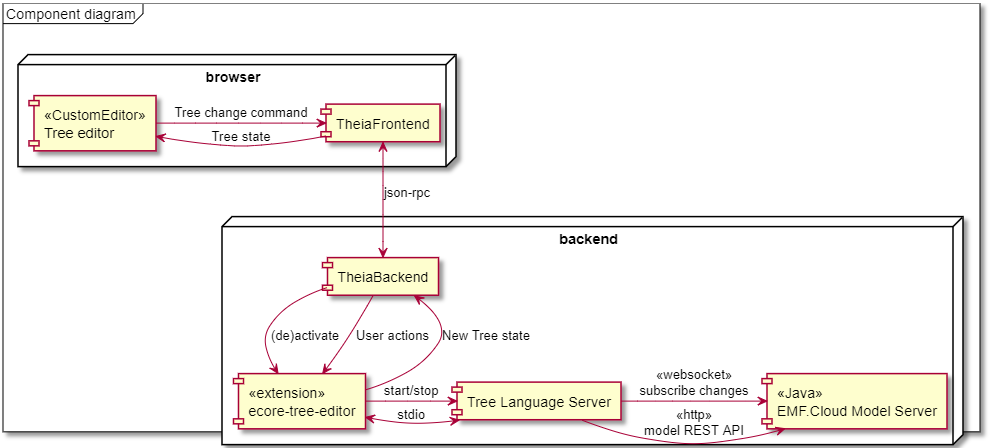
\includegraphics[width=\textwidth]{figures/tree-editor-component-diagram.png}
  \caption[Tree Editor Architecture]{A suggested architecture for a tree editor.}\label{fig:tree-editor-architecture}
\end{figure}

\paragraph*{Sharing a Model Server}
Because multiple extensions might require the same Model Server, an idea (not explored yet) is to have a specific VSCode Extension only for providing this Model Server.
Other extensions can then notify a dependence on this extension, causing it to be installed.
This seems supported at least in VSCode.
The Model Server extension would then provide the details for connecting to it, to other extensions.
It is possible to discover other extensions and get an \gls{API} from them.



% Move the background material for an editor here?
% Keep titles, use pointers in background, detail furhter here.

